% Package
\documentclass[11pt]{article}

\usepackage{amsmath}
\usepackage{cite}
\usepackage{graphicx}
\usepackage[utf8]{inputenc}
\usepackage[T1]{fontenc}
\usepackage{lmodern}
\usepackage[ngerman]{babel}
\usepackage{hyphenat}

\title{ADP Aufgabe 2 Entwurf, Abgabe 1}
\author{Team 1\\Hugo Protsch, Justin Hoffmann}

% Document
\begin{document}

    \maketitle

    \tableofcontents

    \newpage


    \section{Formales}\label{sec:Formales}

    %! suppress = MissingLabel

    \subsection*{Aufgabenaufteilung}
    Der Entwurf für Insertion Sort wurde zusammen entwickelt.\\
    Der Entwurf für Quick Sort wurde von Hugo entwickelt.\\
    Der Entwurf für Heap Sort wurde von Justin entwickelt.
    %! suppress = MissingLabel

    \subsection*{Quellenangaben}
    Es wurden lediglich Vorlesungsmaterialien verwendet.
    %! suppress = MissingLabel

    \subsection*{Bearbeitungszeitraum}
    Der gesamte Arbeitsaufwand für den Entwurf belief sich auf ca. 8 Stunden.
    %TODO Heapsort

    %! suppress = MissingLabel

    \subsection*{Aktueller Stand}
    %! suppress = MissingLabel
    %TODO

    \subsection*{Änderungen des Entwurfes}
    -- nicht zutreffend --


    \section{Insertion Sort}\label{sec:insertion-sort}

    \subsection{Algorithmus}\label{subsec:Ialgorithmus}
    Siehe Abbildung~\ref{fig:insertionS}.
    Bei Insertion Sort wird eine Liste durch das Einfügen von Elementen aus
    einem unsortierten Bereich (zunächst die komplette List) in einen sortieren
    Bereich (zunächst leer, <N1>) sortiert.

    Bei dem Einfügen eines Elements E in den sortierten Bereich muss dabei
    jeweils der Bereich bis zu dem Element durchlaufen werden, hinter das das
    Element E eingefügt werden muss (Siehe \frqq Insert into sorted list\flqq
    Subgraph).

    Somit wird der sortierte Bereich mit jeder Iteration um 1 erhöht <E1>.
    Sobald der sortierte Bereich alle Elemente enthält, wird die Liste
    zurückgegeben.
    Bei der Implementation des Algorithmus auf einfach verkettete Listen
    kann der sortierte und unsortierte Bereich getrennt werden.

    \subsection{Laufzeit}\label{subsec:Ilaufzeit}
    Die erwartete Laufzeit beträgt \(O(n^2)\), da bei jeder Iteration das
    einzufügende Element mit allen noch nicht sortierten Elementen verglichen
    wird.
    Im Fall einer bereits sortierten Liste tritt der Best-Case ein.
    Hierbei müssen nur \(n\) Vergleiche durchgeführt werden.
    Somit beträgt die Laufzeit \(\Theta(n)\).

    Bei der Laufzeitmessung überprüfen wir, ob der gemessene Zusammenhang mit
    dem erwarteten übereinstimmt.
    Dafür verwenden wir für den Best-Case zufällige Listen, im Worst-Case
    bereits sortierte Listen.

    \begin{figure}[hbt]
        \caption{Insertion Sort}
        \centering
        \includegraphics[width = 8cm]{insertionS}\label{fig:insertionS}
    \end{figure}


    \section{Quick Sort}\label{sec:quick-sort}

    \subsection{Algorithmus}\label{subsec:Qalgorithmus}
    Siehe Abbildung~\ref{fig:qsort}.
    Bei Quick Sort wird zunächst willkürlich ein Pivot-Element aus der List
    ausgewählt.

    Anschließend wird die Liste in zwei Teile aufgeteilt: Die Liste L hält alle
    Elemente, die kleiner als das Pivot-Element sind, die Liste R alle
    Elemente, die größer als das Pivot-Element sind.
    Dafür wird die Liste elementweise durchlaufen und jedes Element mit dem
    Pivot-Element verglichen.
    Die Reihenfolge der Elemente in den Listen spielt keine Rolle.
    Das Pivot-Element selber kommt nicht in den Listen vor.

    Da alle Elemente, die kleiner als das Pivot-Element sind und alle Elemente,
    die größer als das Pivot-Element sind, nun getrennt vorliegen, ist die
    Position des Pivots eindeutig als zwischen den Listen L und R bestimmt.
    Somit kann der Algorithmus rekursiv auf die jeweiligen Listen erneut
    angewandt werden.

    Das Pivot-Element wird an die Liste R vorangestellt.
    Die Liste L wird der Liste R, inklusive Pivot, vorangestellt.
    Die Liste ist nun sortiert.

    \begin{figure}[hbt]
        \caption{Insertion Sort}
        \centering
        \includegraphics[width = 8cm]{qsort.pdf}\label{fig:qsort}
    \end{figure}

    \subsection{Laufzeit}\label{subsec:Qlaufzeit}

    Die Laufzeit beträgt im Best-Case \(\Omega (n \cdot \log(n))\), da bei
    gut gewähltem Pivot-Elementen die Anzahl an vergleichen mit jeder
    iteration halbiert wird.
    Wenn das Pivot-Element bei jeder Iteration schlecht gewählt ist (kleinstes
    oder größtes Element in der List), beträgt die Laufzeit \(O(n^2)\), da
    jeweils eine Partition die Größe 1 hat und die Anzahl an vergleichen
    somit nicht reduziert wird.

    Bei der Laufzeitmessung testen wir, ob die Komplexität des implementierten
    Algorithmus mit dem erwarteten übereinstimmt.
    Um den Worst-Case zu überprüfen, nutzten wir bereits sortierte Listen und
    wählen das letzte bzw. erste Element als Pivot-Element.
    Für den Best-Case nutzten wir zufällig generierte Listen.\\
    Wir ermitteln des Weiteren die Elementanzahl, ab der Quicksort schneller
    als Insertion Sort ist.
    Außerdem wird die Implementation mit Erlang List Comprehension der
    eigenen gegenübergestellt.


    \section{Heap Sort}\label{sec:heap-sort}

    \subsection{Algorithmus}\label{subsec:Halgorithmus}
    Siehe Abbildung~\ref{fig:hsort}.


    \begin{figure}[hbt]
        \caption{Heap Sort}
        \centering
        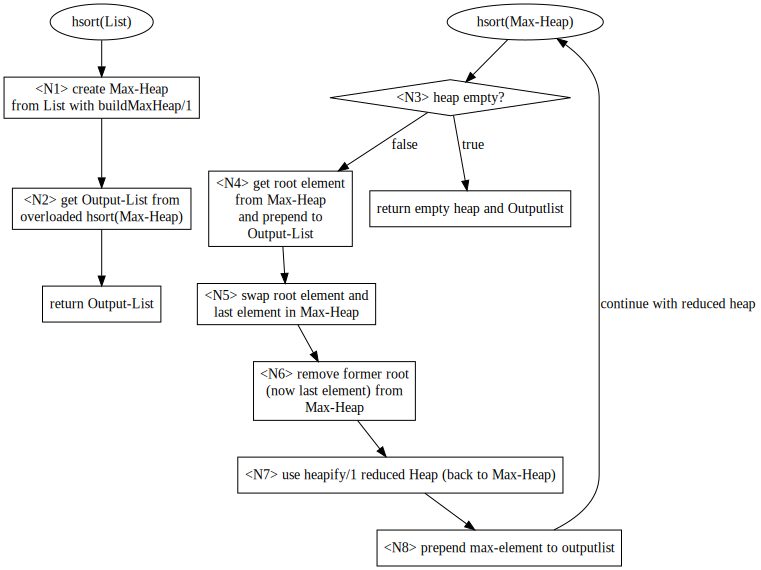
\includegraphics[width = 8cm]{hsort.pdf}\label{fig:hsort}
    \end{figure}

    \begin{figure}[hbt]
        \caption{Heapify}
        \centering
        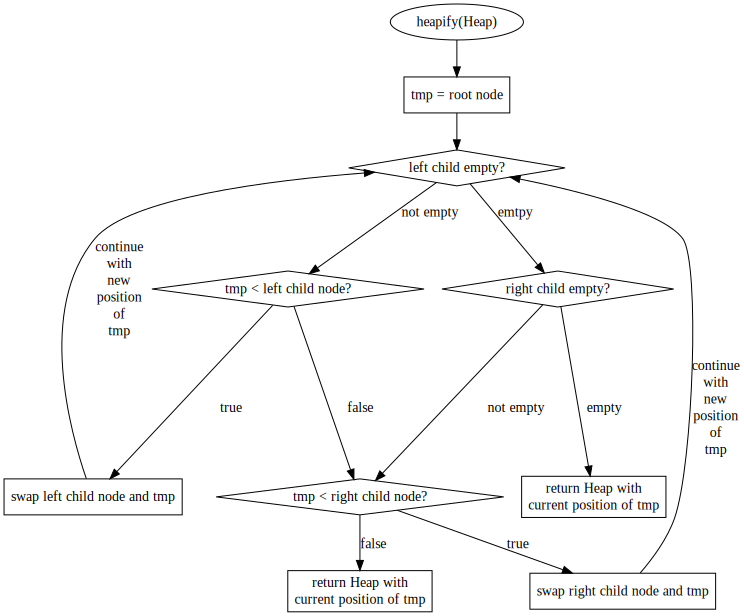
\includegraphics[width = 8cm]{heapify.pdf}\label{fig:heapify}
    \end{figure}

    \subsection{Laufzeit}\label{subsec:Hlaufzeit}

\end{document}
